 \chapter{Operações Numéricas}

 Antes de tratar das operações numéricas e algébricas, vale ressaltar que quando estamos resolvendo uma expressão numérica ou uma expressão algébrica temos vários cálculos para serem feitos sucessivamente, e para tal precisamos obedecer uma ordem de prioridades que é a seguinte:

\begin{multicols}{2}
Resolva em:
\begin{itemize}
\item 1º lugar: raízes e potências;
\item 2º lugar: multiplicação e divisão;
\item 3º lugar: adição e subtração.
\end{itemize}

Priorize cálculos em:
\begin{itemize}
\item 1º lugar: parênteses $($ $)$;
\item 2º lugar: colchetes $[$ $]$;
\item 3º lugar: chaves $\{$ $\}$.
\end{itemize}
\end{multicols}

 \section{Operações em \texorpdfstring{$\N$}{N}}
 No conjunto dos números naturais, que vamos considerar aqui que contém o $0$ (zero) temos bem definida a operação de soma de dois elementos deste conjunto, pois dados $x$, $y \in \N$ temos que existe $z \in \N$ tal que $x+y=z$, e que $y+x=z$. Por exemplo, $2+3=5=3+2$. \emph{Sugestão ao leitor: pense em outros exemplos numéricos.}
 
 Neste conjunto temos um elemento neutro com relação a operação de soma que é o $0$ (zero), pois dado $x \in \N$, temos que $x+0=x=0+x$.
 
 Mas um fato bem importante com relação a operação de soma em $\N$ é que neste conjunto os elementos não possuem inverso com relação a soma, pois dado $x \in \N$ não existe $y \in \N$ tal que $x+y=0$. Por exemplo, dado $3 \in \N$ não existe $y \in \N$ tal que $3 + y=0$. E ainda a "operação de subtração" também não está definida neste conjunto pois, $(4)-(6)=-2$ e $-2 \notin \N$.
 
 No conjunto dos números naturais, temos bem definida também a operação de multiplicação de dois elementos deste conjunto, pois dados $x$, $y \in \N$ temos que existe $z \in \N$ tal que $x \cdot y=z$, e que $y \cdot x=z$. Por exemplo, $2 \cdot 3=6=3 \cdot2$. \emph{Sugestão ao leitor: pense em outros exemplos numéricos.}
 
 Neste conjunto temos um elemento neutro com relação a operação de multiplicação que é o $1$ (um), também chamado de unidade, pois dado $x \in \N$, temos que $x \cdot 1= x= 1 \cdot x$.

 Mas um fato bem importante com relação a operação de multiplicação em $\N$ é que neste conjunto os elementos não possuem inverso com relação a multiplicação, pois dado $x \in \N$ não existe $y \in \N$ tal que $x \cdot y= 1$. Por exemplo, dado $3 \in \N$ não existe $y \in \N$ tal que $3 \cdot y= 1$. Além disso a "operação de divisão" também não está definida neste conjunto pois, $(1)\div (2)= 0,5$ e $0,5 \notin \N$. 
 
  \vskip0.3cm
 
 Portanto em $\N$ as operações de soma $(+)$ e multiplicação $(\cdot)$ possuem as seguintes propriedades:
 
 Soma $(+)$:
 \begin{enumerate}[1)]
 \item Fechamento: dados $x, y \in \N$ temos que $x+y \in \N$;
 \item Associativo: dados $x, y, z \in \N$ temos que $(x+y)+z= x+(y+z)$;
 \item Elemento neutro: existe um elemento $0 \in \N$ tal que $x+0=0+x=x$, para qualquer $x \in \N$;
 \item Comutatividade: dados $x, y \in \N$ temos que $x+y= y+x$.
 \end{enumerate}
 
  Multiplicação $(\cdot)$:
 \begin{enumerate}[1)]
 \item Fechamento: dados $x, y \in \N$ temos que $x \cdot y \in \N$;
 \item Associativo: dados $x, y, z \in \N$ temos que $(x \cdot y) \cdot z= x \cdot (y \cdot z)$;
 \item Elemento neutro: existe um elemento $1 \in \N$ tal que $x \cdot 1= 1 \cdot x= x$, para qualquer $x \in \N$;
 \item Comutatividade: dados $x, y \in \N$ temos que $x \cdot y= y \cdot x$.
 \end{enumerate}
 
 Leis distributivas: $\forall x, y, z \in \N$
 \begin{enumerate}[1)]
 \item $x \cdot (y + z)= x \cdot y + x \cdot z$;
 \item $(x + y) \cdot z= x \cdot z + y \cdot z$.
 \end{enumerate}

 \section{Operações em \texorpdfstring{$\Z$}{Z}}

 Ao operar neste conjunto numérico precisamos lidar com os números negativos e para isso precisamos dominar os jogos de sinais envolvidos nestas operações, então vamos ver alguns exemplos de operações neste conjunto para entender como lidar com os números negativos.

   \vskip0.3cm
   
 \textbf{Adição de números inteiros}

 \begin{itemize}
  \item Na adição de números inteiros com o mesmo sinal, some os números e conserve o sinal;
  \item Na adição de números inteiros com sinais diferentes, subtraia os números e conserve o sinal do maior.
 \end{itemize}

  \begin{enumerate}[1)]
   \item $123 + 7= 130$
   \item $123 - 7= 116$
   \item $-123 + 7 = -116$
   \item $-123 - 7 = -130$
 \end{enumerate}
 
  Neste conjunto temos um elemento neutro com relação a operação de soma que é o $0$ (zero), pois dado $x \in \Z$, temos que $x+0=x=0+x$.
 
 Além disso, como no conjunto dos números inteiros temos todos os números negativos, então todo elemento de $\Z$ possui um inverso aditivo, ou seja, $\forall x \in \Z$ existe um elemento $-x \in \Z$ tal que $x + (-x)=0$. Consequentemente, decorre que neste conjunto a "operação de subtração" esta bem definida, já que dados $x, y \in \Z$ existe $z \in \Z$ tal que $x - y= x+ (-y)= z$.

   \vskip0.3cm
  
 \textbf{Multiplicação e divisão de números inteiros}

  \begin{itemize}
   \item Na multiplicação e divisão de números inteiros com o mesmo sinal o resultado é sempre positivo.
   \item Na multiplicação e divisão de números inteiros com o sinais diferentes o resultado é sempre negativo.
  \end{itemize}

  \begin{multicols}{2}
  \begin{enumerate}[1)]
   \item $8 \cdot 20= 160$
   \item $8 \cdot (-20)= -160$
   \item $-8 \cdot 20= -160$
   \item $(-8) \cdot (-20)= 160$
   \item $45 \div 5= 9$
   \item $45 \div (-5)= -9$
   \item $(-45) \div 5= -9$
   \item $(-45) \div (-5)= 9$
  \end{enumerate}
  \end{multicols}

 Neste conjunto temos um elemento neutro com relação a operação de multiplicação que é o $1$ (um), também chamado de unidade, pois dado $x \in \Z$, temos que $x \cdot 1= x= 1 \cdot x$.

 Mas um fato bem importante com relação a operação de multiplicação em $\Z$ é que neste conjunto os elementos não possuem inverso com relação a multiplicação, pois dado $x \in \Z$ não existe $y \in \Z$ tal que $x \cdot y= 1$. Por exemplo, dado $3 \in \Z$ não existe $y \in \Z$ tal que $3 \cdot y= 1$. Além disso a "operação de divisão" também não está definida neste conjunto pois, $(1)\div (2)= 0,5$ e $0,5 \notin \Z$.
 
   \vskip0.3cm
 
 Portanto em $\Z$ as operações de soma $(+)$ e multiplicação $(\cdot)$ possuem as seguintes propriedades:
 
 Soma $(+)$:
 \begin{enumerate}[1)]
 \item Fechamento: dados $x, y \in \Z$ temos que $x+y \in \Z$;
 \item Associativo: dados $x, y, z \in \Z$ temos que $(x+y)+z= x+(y+z)$;
 \item Elemento neutro: existe um elemento $0 \in \Z$ tal que $x+0=0+x=x$, para qualquer $x \in \Z$;
 \item Elemento inverso: dado $x \in \Z$ qualquer, existe um elemento $-x \in \Z$ tal que $x+(-x)=0$;
 \item Comutatividade: dados $x, y \in \Z$ temos que $x+y= y+x$. 
 \end{enumerate}
 
  Multiplicação $(\cdot)$:
 \begin{enumerate}[1)]
 \item Fechamento: dados $x, y \in \Z$ temos que $x \cdot y \in \Z$;
 \item Associativo: dados $x, y, z \in \Z$ temos que $(x \cdot y) \cdot z= x \cdot (y \cdot z)$;
 \item Elemento neutro: existe um elemento $1 \in \Z$ tal que $x \cdot 1= 1 \cdot x= x$, para qualquer $x \in \Z$;
 \item Comutatividade: dados $x, y \in \Z$ temos que $x \cdot y= y \cdot x$. 
 \end{enumerate}
 
  Leis distributivas: $\forall x, y, z \in \Z$
 \begin{enumerate}[1)]
 \item $x \cdot (y + z)= x \cdot y + x \cdot z$;
 \item $(x + y) \cdot z= x \cdot z + y \cdot z$.
 \end{enumerate}
 
  Como a operação de soma em $\Z$ satisfaz as condições de 1 a 4 acima decorre que $(\Z, +)$ é um grupo aditivo, e por satisfazer a propriedade 5 dizemos que este grupo é abeliano. Como a operação de multiplicação em $\Z$ satisfaz é fechada (1) e associativa (2) e além disso satisfaz as leis distributivas decorre que $\Z$ é um anel. Por valer a comutatividade da multiplicação este anel é comutativo.  


 \section{Operações em \texorpdfstring{$\Q$}{Q}}

 As operações no conjunto dos números Racionais envolvem em particular as operações com frações que possuem algumas particularidades por isso façamos uma rápida retomada destas operações.

 \vskip0.3cm

 \colorbox{azul}{
 \begin{minipage}{0.9\linewidth}
 \begin{center}
  \textbf{Soma:} Dados $x, y, a, b \in \Z$ com $a, b \neq 0$ temos:
 \[\frac{x}{a} + \frac{y}{a}= \frac{x+y}{a} \, \text{ ou}, \ \
  \frac{x}{a} + \frac{y}{b}= \frac{xb + ya}{ab} \]
 \end{center}
 \end{minipage}}

 \vskip0.3cm

 \colorbox{azul}{
 \begin{minipage}{0.9\linewidth}
 \begin{center}
  \textbf{Subtração:} Dados $x, y, a, b \in \Z$ com $a, b \neq 0$ temos:
 \[\frac{x}{a} - \frac{y}{a}= \frac{x-y}{a} \, \text{ ou}, \ \
 \frac{x}{a} - \frac{y}{b}= \frac{xb - ya}{ab} \]
 \end{center}
 \end{minipage}}

 \vskip0.3cm

 \begin{exem}
  \textbf{Soma e subtração de frações com mesmo denominador:}

   Quando os denominadores das frações são iguais, mantemos o denominador e operamos os numeradores.
    \vskip0.3cm
   \[\frac{3}{5} + \frac{1}{5}= \frac{3+1}{5}= \frac{4}{5} .\]
    \vskip0.3cm
   \[\frac{3}{5} - \frac{1}{5}= \frac{3-1}{5}= \frac{2}{5} .\]
 \end{exem}

 \begin{exem}
 \textbf{Soma e subtração de frações com denominadores diferentes:}

   Quando os denominadores das frações são diferentes podemos simplesmente multiplicar os denominadores ou calcular o mínimo múltiplo comum entre eles (MMC), a vantagem da segunda opção é que o MMC é menor ou igual ao produto, como podemos ver no exemplo:
    \vskip0.3cm
   \[\frac{2}{4} + \frac{3}{10}= \frac{10 \cdot 2 + 4 \cdot 3}{4 \cdot 10}= \frac{20 + 12}{40}= \frac{32}{40}= \frac{4}{5} .\]
    \vskip0.3cm
   \[\frac{2}{4} - \frac{3}{10}= \frac{10 \cdot 2 - 4 \cdot 3}{4 \cdot 10}= \frac{20 - 12}{40}= \frac{8}{40}= \frac{1}{5} .\]
    \vskip0.3cm
   Observamos que o $MMC(4, 10)= 20$, assim,
    \vskip0.3cm
   \[\frac{2}{4} + \frac{3}{10}= \frac{5 \cdot 2 + 2 \cdot 3}{20}= \frac{10+6}{20}= \frac{16}{20}=\frac{4}{5} .\]
    \vskip0.3cm
   \[\frac{2}{4} - \frac{3}{10}= \frac{5 \cdot 2 - 2 \cdot 3}{20}= \frac{10 - 6}{20}= \frac{4}{20}=\frac{1}{5} .\]
 \end{exem}


 \vskip0.5cm

 \colorbox{azul}{
 \begin{minipage}{0.9\linewidth}
 \begin{center}
  \textbf{Multiplicação:} Dados $a, b, c, d \in \Z$ com $b, d \neq 0$ temos:
 \[\frac{a}{b} \cdot \frac{c}{d}= \frac{a \cdot c}{b \cdot d} \]
 \end{center}
 \end{minipage}}

 \vskip0.3cm
 \begin{exem}
  \textbf{Multiplicação de fração:} na multiplicação devemos multiplicar numerador por numerador e denominador por denominador.
   \[\frac{2}{3} \cdot \frac{6}{4}= \frac{2 \cdot 6}{3 \cdot 4}= \frac{12}{12}= 1 \]
   \[2 \cdot \frac{5}{3}= \frac{2 \cdot 5}{3}= \frac{10}{3}\]
 \end{exem}

 \vskip0.3cm

 \colorbox{azul}{
 \begin{minipage}{0.9\linewidth}
 \begin{center}
  \textbf{Divisão:} Dados $a, b, c, d \in \Z$ com $b, c, d \neq 0$ temos:
 \[\frac{a}{b} \div \frac{c}{d}= \frac{a}{b} \cdot \frac{d}{c} \]
 \end{center}
 \end{minipage}}

 \vskip0.3cm
 \begin{exem}
  \textbf{Divisão de fração:} na divisão conservamos a primeira fração e multiplicamos pelo inverso da segunda.
   \[\frac{2}{3} \div \frac{1}{6}= \frac{2}{3} \cdot \frac{6}{1}= \frac{2 \cdot 6}{3 \cdot 1}= \frac{12}{3}= 4 \]
   \[\frac{4}{\left(\frac{2}{3}\right)}= \frac{4}{1} \cdot \frac{3}{2}= \frac{12}{2}=6\]
 \end{exem}

 Como visto anteriormente existe uma cópia do conjunto dos números inteiros dentro do conjunto dos números racionais, portanto todas as operações de soma e multiplicação dos números inteiros funcionam da mesma forma no conjunto dos racionais, portanto o jogo de sinais para soma e multiplicação nos racionais são iguais aos jogos de sinais nos inteiros, por isso não iremos detalhar aqui. Mas vale chamar atenção para alguns detalhes do conjunto $\Q$.
 
   Neste conjunto temos um elemento neutro com relação a operação de soma que é o $0$ (zero), pois dado $x \in \Q$, temos que $x+0= x= 0+x$.
 
 Além disso, como no conjunto dos números racionais temos todos os números negativos, então todo elemento de $\Q$ possui um inverso aditivo, ou seja, $\forall x \in \Q$ existe um elemento $-x \in \Q$ tal que $x + (-x)=0$. Consequentemente, decorre que neste conjunto a "operação de subtração" esta bem definida, já que dados $x, y \in \Q$ existe $z \in \Q$ tal que $x - y= x+ (-y)= z$.
 
 Neste conjunto temos um elemento neutro com relação a operação de multiplicação que é o $1$ (um), também chamado de unidade, pois dado $x \in \Q$, temos que $x \cdot 1= x= 1 \cdot x$.

 Além disso, com relação a operação de multiplicação em $\Q$, vale obervar que neste conjunto os elementos diferentes de $0$ (zero) possuem inverso com relação a multiplicação, pois dado $x \neq 0 \in \Q$ existe $x^{-1}= \frac{1}{x} \in \Q$ tal que $x \cdot x^{-1}= 1$. Por exemplo, dado $3 \in \Q$ existe $3^{-1}= \frac{1}{3} \in \Q$ tal que $3 \cdot \frac{1}{3}= 1$. Portanto a "operação de divisão" está definida neste conjunto.
 
   \vskip0.3cm
 
 Portanto em $\Q$ as operações de soma $(+)$ e multiplicação $(\cdot)$ possuem as seguintes propriedades:
 
 Soma $(+)$:
 \begin{enumerate}[1)]
 \item Fechamento: dados $x, y \in \Q$ temos que $x+y \in \Q$;
 \item Associativo: dados $x, y, z \in \Q$ temos que $(x+y)+z= x+(y+z)$;
 \item Elemento neutro: existe um elemento $0 \in \Q$ tal que $x+0=0+x=x$, para qualquer $x \in \Q$;
 \item Elemento inverso: dado $x \in \Q$ qualquer, existe um elemento $-x \in \Q$ tal que $x+(-x)=0$;
 \item Comutatividade: dados $x, y \in \Q$ temos que $x+y= y+x$. 
 \end{enumerate}
 
  Multiplicação $(\cdot)$:
 \begin{enumerate}[1)]
 \item Fechamento: dados $x, y \in \Q$ temos que $x \cdot y \in \Q$;
 \item Associativo: dados $x, y, z \in \Q$ temos que $(x \cdot y) \cdot z= x \cdot (y \cdot z)$;
 \item Elemento neutro: existe um elemento $1 \in \Q$ tal que $x \cdot 1= 1 \cdot x= x$, para qualquer $x \in \Q$;
 \item Elemento inverso: dado $x \in \Q$ qualquer, existe um elemento $x^{-1} \in \Q$ tal que $x \cdot x^{-1}= 1$;
 \item Comutatividade: dados $x, y \in \Q$ temos que $x \cdot y= y \cdot x$. 
 \end{enumerate}
 
  Leis distributivas: $\forall x, y, z \in \Q$
 \begin{enumerate}[1)]
 \item $x \cdot (y + z)= x \cdot y + x \cdot z$;
 \item $(x + y) \cdot z= x \cdot z + y \cdot z$.
 \end{enumerate}
 
  Como a operação de soma em $\Q$ satisfaz as condições de 1 a 4 acima decorre que $(\Q, +)$ é um grupo aditivo, e por satisfazer a propriedade 5 dizemos que este grupo é abeliano. Analogamente, como a operação de multiplicação em $\Q$ satisfaz as propriedades de 1 a 4 decorre que $(\Q, \cdot)$ é um grupo multiplicativo, e por satisfazer a propriedade 5 é um grupo abeliano. Além disso, como a operação de multiplicação em $\Q$ é fechada (1) e associativa (2) e além disso satisfaz as leis distributivas decorre que $\Q$ é um anel. 
  
  Além disso, $\Q$ com as operações de soma e multiplicação, como definidas é também um corpo. Vale aqui observar que todo conjunto com duas operações, soma e multiplicação, bem definidas, satisfazendo as propriedade de 1 a 5 respectivamente, e as leis de distributividade são denominados \emph{corpos}. 
 
 \section{Operações em \texorpdfstring{$\I$}{I} e \texorpdfstring{$\R$}{R}}
 
 Para finalizar, lembramos que há uma cópia dos números racionais dentro do conjunto dos números reais, portanto todas as propriedades das operações em $\Q$ continuam válidas para estes números dentro de $\R$. Assim, para compreendermos como funcionam as operações em $\R= \Q \cup \I$ precisamos aprender a operar em $\I$. As operações entre números irracionais que são raízes de alguma ordem de outros números serão discutidas no próximo capítulo, as operações entre números irracionais como por exemplo $\pi + e$, costumamos deixar indicadas, por este motivo não precisamos detalhar este caso.
 
 Mas destacamos que em $\R$ as operações de soma (adição) $(+)$ e multiplicação $(\cdot)$ possuem as seguintes propriedades:
 
 Soma (adição) $(+)$:
 \begin{enumerate}[1)]
 \item Fechamento: dados $x, y \in \R$ temos que $x+y \in \R$;
 \item Associativo: dados $x, y, z \in \R$ temos que $(x+y)+z= x+(y+z)$;
 \item Elemento neutro: existe um elemento $0 \in \R$ tal que $x+0=0+x=x$, para qualquer $x \in \R$;
 \item Elemento inverso: dado $x \in \R$ qualquer, existe um elemento $-x \in \Q$ tal que $x+(-x)=0$;
 \item Comutatividade: dados $x, y \in \R$ temos que $x+y= y+x$. 
 \end{enumerate}
 
  Multiplicação $(\cdot)$:
 \begin{enumerate}[1)]
 \item Fechamento: dados $x, y \in \R$ temos que $x \cdot y \in \R$;
 \item Associativo: dados $x, y, z \in \R$ temos que $(x \cdot y) \cdot z= x \cdot (y \cdot z)$;
 \item Elemento neutro: existe um elemento $1 \in \R$ tal que $x \cdot 1= 1 \cdot x= x$, para qualquer $x \in \R$;
 \item Elemento inverso: dado $x \in \R$ qualquer, existe um elemento $x^{-1} \in \R$ tal que $x \cdot x^{-1}= 1$;
 \item Comutatividade: dados $x, y \in \R$ temos que $x \cdot y= y \cdot x$. 
 \end{enumerate}
 
  Leis distributivas: $\forall x, y, z \in \R$
 \begin{enumerate}[1)]
 \item $x \cdot (y + z)= x \cdot y + x \cdot z$;
 \item $(x + y) \cdot z= x \cdot z + y \cdot z$.
 \end{enumerate}
 
   Quando um conjunto tem duas operações satisfazendo as propriedades acima ele costuma ser chamado de \emph{corpo}. Portanto, $\R$ é um \emph{corpo}. Este e outros corpos são utilizados em disciplinas como Álgebra Linear.
   
   Só por curiosidade, um outro exemplo de corpo é o conjunto $\Z_2= \{0, 1\}$, no qual definimos $1+1=0$, pois neste conjunto as operações de adição e multiplicação satisfazem todas as propriedades mencionadas anteriormente.

 \chapter{Potenciação}

 \section{Potência com expoente inteiro}

 \vskip0.3cm

 \colorbox{azul}{
 \begin{minipage}{0.9\linewidth}
 \begin{center}
  Dados dois números $a \in \R$ e $b \in \N$ definimos:
 \[a^b= \underbrace{a \cdot a \cdot \cdots \cdot a}_{b \text{ vezes}} .\]
  Dizemos que $a$ é a base da potência e $b$ o expoente. Lê-se: $a$ elevado a $b$.
 \end{center}
 \end{minipage}}

 \vskip0.3cm

 \begin{exem}
 Observe que neste caso o expoente é um número natural, e portanto positivo, como por exemplo:

  $2^3= 2 \cdot 2 \cdot 2= 8$;

  $2^4=2 \cdot 2 \cdot 2 \cdot  2= 16$;

  $3^2= 3 \cdot 3= 9$;

  $5^3= 5 \cdot 5 \cdot 5= 125$.

  Este é o único caso em que temos a potência definida, se tivermos qualquer outro número no expoente precisamos fazer recair nesta situação.
 \end{exem}


 \vskip0.3cm

 \colorbox{azul}{
 \begin{minipage}{0.9\linewidth}
 \begin{center}
   Dados dois números $a \in \R$ e $b \in \Z$ definimos:
 \[a^b= \underbrace{a \cdot a \cdot \cdots \cdot a}_{b \text{ vezes}}, \text{ para } b\geq0, \text{ esta situação está inclusa no caso anterior};\]
 \[a^{-b}= \frac{1}{a^b}= \underbrace{\frac{1}{a} \cdot \frac{1}{a} \cdot \cdots \cdot \frac{1}{a}}_{b \text{ vezes}}, \text{ para } b>0 ;\]
 \[\frac{1}{a^{-b}}= a^b, \text{ para } b>0;\]
 \end{center}
 \end{minipage}}

 \vskip0.3cm

 \begin{exem}
 Vejamos agora alguns exemplos em que o expoente é um número negativo:
 \begin{eqnarray*}
  2^{-1}= \frac{1}{2^{1}}= \frac{1}{2}; \\
  2^{-3}= \frac{1}{2^3}= \frac{1}{8}; \\
  \frac{1}{3^{-2}}= 3^2= 3 \cdot 3= 9; \\
  \left( \frac{8}{22} \right)^{-2}= \left( \frac{22}{8} \right)^{2}= \frac{22}{8} \cdot \frac{22}{8}= \frac{484}{64}.
 \end{eqnarray*}
 Note que em todos os exemplos acima o que fizemos foi "inverter" a fração, e com isso deixamos os expoentes positivos, e então basta aplicar a definição de potência.

 \end{exem}

 
 Se $a, b \in \R$, $m, n \in \N$, então valem as seguintes propriedades:
 \begin{enumerate}[P1)]
 \item $a^m \cdot a^n= a^{m + n}$;
 \item $a^m \div a^n= a^{m - n}$, para $a \neq 0$;
 \item $(a^m)^n= a^{m \cdot n}$;
 \item $(a \cdot b)^n= a^n \cdot b^n$;
 \item $\left(\frac{a}{b}\right)^n= \frac{a^n}{b^n}$, para $b \neq 0$;
 \item $a^{-n}= \frac{1}{a^n}$, para $(a \neq 0)$;
 \item $\left(\frac{a}{b} \right)^{-n}= \left(\frac{b}{a} \right)^{n}$, para $a \neq 0$ e $b \neq 0$;
 \end{enumerate}
 
  \vskip0.3cm

 \colorbox{amarelo}{
 \begin{minipage}{0.9\linewidth}
 \begin{center}
 Aqui é importante observar que:
 \begin{align*}
 & \nexists 0^0 & & a^1= a, \forall a \in \R & & a^0= 1, \forall a \in \R & & 1^a= 1, \forall a \in \R
 \end{align*}
 \end{center}
 \end{minipage}}
 
\vskip0.3cm 

 \section{Raiz}
 
 Dados um número real $a \geq 0$ e um número natural $n$, existe um número real positivo ou nulo $b$ tal que $b^n= a$. O número real $b$ é chamado de raiz enézima de $a$, ou raiz de ordem $n$ de $a$ e indicaremos por $\sqrt[n]{a}$.
 
 \begin{obs}
 Da definição decorre que $(\sqrt[n]{a})^n=a$.
 \end{obs}
 
 \begin{obs}
 Note que de acordo com a definição dada $\sqrt{36}= 6$ e não $\sqrt{36}= \pm 6$.
 \end{obs}
 
 \begin{obs}
 Muita atenção ao calcular a raiz quadrada de um quadrado perfeito:
 \[\sqrt{a^2}= |a| \ . \]
 \end{obs}
 
 Se $a, b \in \R_{+}$, $m \in \Z$, $n \in \N^{*}$, e $p \in \N^{*}$, então valem as seguintes propriedades:
 \begin{enumerate}[R1)]
 \item $\sqrt[n]{a^m}= \sqrt[n \cdot p]{a^{m\cdot p}}$;
 \item $\sqrt[n]{a \cdot b}= \sqrt[n]{a} \cdot \sqrt[n]{b}$;
 \item $\sqrt[n]{\frac{a}{b}}= \frac{\sqrt[n]{a}}{\sqrt[n]{b}}$, para $b \neq 0$;
 \item $(\sqrt[n]{a})^m= \sqrt[n]{a^m}$;
 \item $\sqrt[p]{\sqrt[n]{a}}= \sqrt[p \cdot n]{a}$.
 \end{enumerate}

 \section{Potência com expoente racional}
 
 A radiciação pode ser entendida como uma potência com expoente racional, a partir da seguinte definição.
 \vskip0.3cm

 \colorbox{azul}{
 \begin{minipage}{0.9\linewidth}
 \begin{center}
  Dados dois números $a \in \R^{*}_{+}$ e $\frac{m}{n} \in \Q$ ($m \in \Z$ e $n \in N^{*}$), definimos:
 \[a^{\frac{m}{n}}= \sqrt[n]{a^m}, \text{ para } \frac{m}{n} >0 ;\]
 \[a^{-\frac{m}{n}}= \frac{1}{a^{\frac{m}{n}}}= \frac{1}{\sqrt[n]{a^m}},  \text{ para } \frac{m}{n} >0.\]
 \end{center}
 \end{minipage}}

 \vskip0.3cm
 
 Entendida a radiciação como potência são válidas aqui todas as propriedades de potência com expoente inteiro listadas anteriormente.

 \begin{exem}
  Vejamos agora alguns exemplos de potência com expoente sendo um número racional ($b \in \mathbb{Q}$):
  \begin{eqnarray*}
   4^{\frac{1}{2}}= \sqrt{4}= 2 \\
   8^{\frac{1}{3}}= \sqrt[3]{8^1}= \sqrt[3]{2^{3}}= 2 \\
   27^{\frac{2}{6}}= \sqrt[6]{27^2}= \sqrt[6]{729}= \sqrt[6]{3^6}= 3\\
   9^{-\frac{1}{2}}= \frac{1}{9^{\frac{1}{2}}}= \frac{1}{\sqrt{9}}= \frac{1}{3} \\
   \left(\frac{4}{9}\right)^{-\frac{1}{2}}= \left(\frac{9}{4}\right)^{\frac{1}{2}}= \sqrt{\left(\frac{9}{4}\right)}=\frac{\sqrt{9}}{\sqrt{4}}= \frac{3}{2} \\
   \frac{2}{3^{-2}}= 2 \cdot \frac{1}{3^{-2}}= 2 \cdot 3^{2}= 2 \cdot 9= 18
  \end{eqnarray*}

 \end{exem}
 
 \section{Potência com expoente irracional}
 
 Dados um número real $a > 0$ e um número irracional $\alpha$, podemos construir por meio de aproximações sucessivas de potências de $a$ com expoente racional, um único número real positivo $a^{\alpha}$ que é potência de base $a$ e expoente irracional $\alpha$.
 
 Esse método é decorre do fato que um número irracional pode ser aproximado por falta ou por excesso por sequências de números racionais, e potências com expoentes racionais estão bem definidas, então podemos utilizar estes dois fatos e definir potências com expoente irracionais que satifazem todas as propriedades de potências já descritas. Vejamos um exemplo:
 
 \begin{exem}
 Consideremos o número irracional $\sqrt{2}= 1,414213562\ldots$. Observe que podemos aproximar $\sqrt{2}$ por falta ou por excesso pelos seguintes números racionais:
 
 \begin{multicols}{2}
 por falta:
 \begin{eqnarray*}
 1 &=& 1\\
 1,4 &=& \dfrac{14}{10} \\
 1,41 &=& \dfrac{141}{100} \\
 1,414 &=& \dfrac{1414}{1000} \\
 1,4142 &=& \dfrac{14142}{1000}
 \end{eqnarray*}
 
 por excesso:
 \begin{eqnarray*}
 2 &=& 2\\
 1,5 &=& \dfrac{15}{10} \\
 1,42 &=& \dfrac{142}{100} \\
 1,415 &=& \dfrac{1415}{1000} \\
 1,4143 &=& \dfrac{14143}{1000}
 \end{eqnarray*}
 \end{multicols} 
 
 Assim podemos definir o valor de $13^{\sqrt{2}}$ por aproximação por falta ou por excesso de potências de base $13$, da seguinte forma:
 
 por falta:
 \begin{eqnarray*}
 13^1 =& 13^1 &= 13\\
 13^{1,4} =& 13^{\frac{14}{10}} =& 36,267756667 \\
 13^{1,41} =& 13^{\frac{141}{100}} =& 37,210039132 \\
 13^{1,414} =& 13^{\frac{1414}{1000}} =& 37,59377174 \\
 13^{1,4142} =& 13^{\frac{14142}{1000}} =& 37,613061911
 \end{eqnarray*}
 
 por excesso:
 \begin{eqnarray*}
 13^{2} =& 13^{2} =& 169 \\
 13^{1,5} =& 13^{\frac{15}{10}} =& 46,872166581 \\
 13^{1,42} =& 13^{\frac{142}{100}} =& 38,176803296\\
 13^{1,415} =& 13^{\frac{1415}{1000}} =& 37,69032163 \\
 13^{1,4143} =& 13^{\frac{14143}{10000}} =& 37,622710708
 \end{eqnarray*}
 
 Portanto $13^{\sqrt{2}} \approx 37,6$.
 \end{exem}

 Se $a=0$ e $\alpha$ é irracional e positivo, definimos $0^{\alpha}=0$.
 
 \begin{obs}
 Se $a=1$ então $1^{\alpha}= 1, \forall \alpha$ irracional.
 \end{obs}
 
 \begin{obs}
 Se $a < 0$ e $\alpha$ é irracional e positivo então o símbolo $a^{\alpha}$ não tem significado.
 \end{obs}
 
 \begin{obs}
 Se $\alpha$ é irracional e negativo $(\alpha < 0)$ então $0^{\alpha}$ não tem significado.
 \end{obs}
 
 \begin{obs}
 Para as potências de expoente irracional são válidas as propriedades de potências com expoente racional.
 \end{obs}

 \section{Potência com expoente real}
 
 Considerando que já foram definidas anteriormente as potências de base $a \in \R^{*}_{+}$ e expoente $b$ ($b$ racional ou  irracional) então já está definida a potência $a^b$ com $a \in \R^{*}_{+}$ e $b \in \R$.
 
 \begin{obs}
 Toda potência de base real e positiva e expoente real é um número real positivo.
 \[a> 0 \Rightarrow a^b > 0 \ .\]
 \end{obs}
 
  Se $a, b \in \R^{*}_{+}$, $m, n \in \R$, então valem as seguintes propriedades:
 \begin{enumerate}[P1)]
 \item $a^m \cdot a^n= a^{m + n}$;
 \item $a^m \div a^n= a^{m - n}$, para $a \neq 0$;
 \item $(a^m)^n= a^{m \cdot n}$;
 \item $(a \cdot b)^n= a^n \cdot b^n$;
 \item $\left(\frac{a}{b}\right)^n= \frac{a^n}{b^n}$, para $b \neq 0$;
 \item $a^{-n}= \frac{1}{a^n}$, para $(a \neq 0)$;
 \item $\left(\frac{a}{b} \right)^{-n}= \left(\frac{b}{a} \right)^{n}$, para $a \neq 0$ e $b \neq 0$;
 \end{enumerate}
 


 \chapter{Operações Algébricas}

 Expressões algébricas são expressões matemáticas que envolvem números, letras e operações.

 Como por exemplo:

 \begin{eqnarray*}
  2x=4,\\
  x^2+1=0,\\
  x(x+3)=5,\\
  2x+3y=17,\\
  x^2 + 2y + 3z -4= 52, \\
  \frac{14x + 8y}{2x}= 3, \\
  \frac{2}{5}x^3 + 3\sqrt{x^4}= 67, \\
  5x(x+3)-4x(2-x)=7.
 \end{eqnarray*}

 Nestas expressões as letras que aparecem são chamadas de \textbf{variáveis}, e os números que aparecem multiplicando uma letra são chamados de \textbf{coeficientes}.

 As expressões algébricas são utilizadas dentre outras coisas, para descrever uma situação problema na qual não conhecemos todos os valores envolvidos, representar uma fórmula, ou expressar uma equação. Devido a sua importância nas exatas precisamos compreender como se comportam as operações presentes nas expressões algébricas, em outras palavras, como fazer contas com letras.

 \vskip0.3cm

 \textbf{Adição e subtração}

 Podemos somar somente letras iguais e com mesmo expoente. Como por exemplo:

 \begin{itemize}
  \item $2x + x= (2+1)x= 3x$
  \item $x^2 - 3x^2= (1-3)x^2= -2x^2$
  \item $2x + y + 5x^2 + 7y - 3x= 5x^2 + (2-3)x + (1+7)y= 5x^2 - 1x + 8y$
  \item $3(x+ 4y-2)= 3x + 3.4y - 3.2= 3x + 12y - 6$
 \end{itemize}

  \vskip0.3cm

 \textbf{Multiplicação}

 Na multiplicação devemos sempre multiplicar coeficiente por coeficiente e letra por letra. Sendo que no caso das letras serem iguais, devemos manter a letra e somar seus expoentes, e no caso das letras serem diferentes apenas fazemos a associação das duas letras. Como mostram os seguintes exemplos:

  \begin{itemize}
   \item $x \cdot x = x^{1+1}= x^2$
   \item $x \cdot x^2= x^{1+2}= x^3$
   \item $x \cdot 2y= (1 \cdot 2)xy= 2xy$
   \item $3x \cdot 2x^2y= (3 \cdot 2)x^{1+2}y= 6x^3y$
   \item $4x^4 \cdot \frac{1}{2}x^{-2}= (4 \cdot \frac{1}{2})x^{4-2}= 2x^2$
   \item $(x - 1) \cdot (x - 2)= x(x-2) - 1(x-2)= x^2 -2x -x +2= x^2 - 3x + 2$
  \end{itemize}

  \vskip0.3cm

   \textbf{Divisão}

   Na divisão devemos sempre dividir coeficiente por coeficiente e letra por letra. Sendo que no caso das letras serem iguais, devemos manter a letra e subtrair seus expoentes, e no caso das letras serem diferentes apenas fazemos a associação das duas letras. Como mostram os seguintes exemplos:

  \begin{itemize}
   \item $x \div x= x^{1-1}= x^0= 1$
   \item $x \div x^2= x^{1-2}= x^{-1}= \frac{1}{x}$
   \item $2y \div x= 2\frac{y}{x}$
   \item $4y^3 \div 2y^2= \frac{4}{2} \cdot \frac{y^3}{y^2}= 2y^{3-2}= 2y$
   \item $\frac{x^2yz^3}{x^2y^3z^2}= x^{2-2}y^{1-3}z^{3-2}= x^0 y^{-2}z^{1}= \frac{z}{y^2}$
   \item $\frac{(x+3) \cdot (x-1)}{(x-1)\cdot (2x+3)}= \frac{x+3}{2x+3}$
  \end{itemize}

 \vskip0.3cm

  \textbf{Potenciação}

  Na potenciação devemos aplicar o expoente ao coeficiente e à incógnita, obedecendo as propriedades de potência.

    \begin{itemize}
     \item $(2x)^2= 2^2 \cdot x^2= 4x^2$
     \item $(3x^2)^3= 3^3 \cdot x^{2\cdot 3}= 27x^6$
     \item $\left(\frac{3a^2}{4}\right)^2= \frac{3^2 a^{2 \cdot 2}}{4^2}= \frac{9a^4}{16}$
    \end{itemize}

  \vskip0.3cm

  \textbf{Radiciação}

  Na radiciação devemos extrair a raiz do coeficiente e da incógnita. Observamos que extrair a raiz da incógnita é equivalente a dividir seu expoente pelo índice da raiz.
    \begin{itemize}
     \item $\sqrt{x}= x^{\frac{1}{2}}$
     \item $\sqrt{x^4}= (x^4)^{\frac{1}{2}}= x^{\frac{4}{2}}= x^2$
     \item $\sqrt[3]{8x^6}= \sqrt[3]{8} \cdot \sqrt[3]{x^6}= 2 x^{\frac{6}{3}}= 2x^2$
     \item $\sqrt{\frac{2x^2}{16}}= \frac{\sqrt{2x^2}}{\sqrt{16}}= \frac{|x|\sqrt{2}}{4}$
     \item $\sqrt{x^2}= |x|$
    \end{itemize}

 \vskip0.3cm

  \textbf{Fatoração das expressões algébricas}

 \vskip0.3cm

 A fatoração das expressões algébricas, é o que nos permite escrever a expressão como um produto de dois termos, ela é utilizada principalmente na resolução de equações, para acelerar o processo de resolução.

 Os seguintes casos de fatoração são os mais utilizados:
 \begin{itemize}
  \item Fator em comum: $x^2 + x= x(x + 1)$; $4x^2 + 6= 2(2x^2 + 3)$
  \item Agrupamento: $ax + bx + ay + by= (a+b)x+(a+b)y= (a+b)(x+y)$
  \item Trinômio quadrado perfeito (+): $(a + b)^2= a^2 + 2ab + b^2$
  \item Trinômio quadrado perfeito (-): $(a - b)^2= a^2 - 2ab + b^2$
  \item Diferença de dois quadrados: $(a + b) \cdot (a - b)= a^2 - b^2$
  \item Cubo perfeito (+): $(a+b)^3= a^3 + 3a^2b + 3ab^2 + b^3$
  \item Cubo perfeito (-): $(a-b)^3= a^3 - 3a^2b + 3ab^2 - b^3$
 \end{itemize}
 
 \newpage
 \section{Polinômios}
 
  \vskip0.3cm
 \colorbox{azul}{
 \begin{minipage}{0.9\linewidth}
 \begin{center}
  Seja $K= \R \text{ ou } \C$. Um polinômio $p$ na incógnita $x$ e com coeficientes em $K$ (simbolicamente, $p \in K[x]$) é uma expressão da forma
  \[p(x)= a_nx^n + a_{n-1}x^{n-1}+ \ldots + a_1x+ a_0= \sum_{i=0}^{n} a_ix^i ,\]
  em que os coeficientes $a_n, \ldots, a_0 \in K$, $a_n \neq 0$ e $n \in \N$. O número natural $n$ é chamado de grau do polinômio $p$, e escreve-se $gr(p)= n$. O termo $a_0$ é denominado termo constante de $p$.
 \end{center}
 \end{minipage}}
 \vskip0.3cm
 
 \begin{obs}
 Os termos polinômio e função polinomial serão considerados como sinônimos e utilizados sem distinção no decorrer deste texto.
 \end{obs}
 
 Uma função polinomial de grau $0$ é uma função constante; uma função polinomial de grau $1$ é uma função linear (ou, função afim); uma função polinomial de grau $2$ é uma função quadrática.
 
 Por simplicidade, a partir de agora iremos considerar nossos polinômios sobre $\R$, porém esta teoria pode ser estendida sem muita dificuldade para o corpo dos números complexos.
 
 \begin{defi}
 Dados um número real $k$ e o polinômio $p(x)= a_nx^n + a_{n-1}x^{n-1}+ \ldots + a_1x+ a_0$, chama-se \emph{valor numérico de $p$ em $k$} ao valor:
 \[p(k)= a_nk^n + a_{n-1}k^{n-1}+ \ldots + a_1k+ a_0 \ .\]
 \end{defi}
 
\begin{exem}
Por exemplo, se considerarmos o polinômio $p(x)= x^2 + 7x+10$, temos os seguintes valores numéricos para $p$:
\begin{eqnarray*}
p(-6)&=& (-6)^2 + 7(-6) +10= 4\\
p(-5)&=& (-5)^2 + 7(-5) +10= 0\\
p(-4)&=& (-4)^2 + 7(-4) +10= -2\\
p(-2)&=& (-2)^2 + 7(-2) +10= 0\\
p(0)&=& 0^2 + 7 \cdot 0 +10= 10\\
\end{eqnarray*}
\end{exem} 
 
 \begin{defi}
 Em particular, se $k$ é um número real tal que $p(k)= 0$, dizemos que $k$ é uma \emph{raiz} ou \emph{um zero} de $p$.
 \end{defi}
 
 \begin{exem}
 Portanto no exemplo anterior temos que $k_1= -5$ e $k_2=-2$ são raízes do polinômio $p(x)= x^2 + 7x+10$.
 \end{exem}
 
  \begin{defi}
  O polinômio nulo (ou identicamente nulo) é um polinômio da forma $p(x)= 0x^n +0x^{n-1}+ \ldots + 0x+ 0$, ou simplesmente, $p(x)= 0$. Por convenção, o grau deste polinômio será indefinido.
 \end{defi}
 
 
  \begin{teo}
  Sejam $p$ e $q$ dois polinômios em $K$, dados por:
  \[p(x)= a_nx^n + a_{n-1}x^{n-1}+ \ldots + a_1x+ a_0= \sum_{i=0}^{n} a_ix^i\]
  \[q(x)= b_nx^n + b_{n-1}x^{n-1}+ \ldots + b_1x+ b_0= \sum_{i=0}^{n} b_ix^i\]
  temos que $p=q \Leftrightarrow a_i= b_i$, para todo $i \in \{0, 1, 2, \cdots, n\}$.
 \end{teo}
 
 \begin{dem}
 Para todo $x \in \R$, temos:
 \[a_i= b_i \Leftrightarrow a_i - b_i=0 \Leftrightarrow (a_i - b_i)x^i=0 \Leftrightarrow \sum_{i=0}^{n}(a_i - b_i)x^i= 0 \Leftrightarrow\]
 \[ \sum_{i=0}^{n}a_i x^i - \sum_{i=0}^{n}b_i x^i = 0 \Leftrightarrow \sum_{i=0}^{n}a_i x^i = \sum_{i=0}^{n}b_i x^i \Leftrightarrow p(x)= q(x)\]

 \end{dem}
 
  Este Teorema mostra que, quando escrevemos um polinômio $p$ na forma 
 \[p(x)= a_nx^n + a_{n-1}x^{n-1}+ \ldots + a_1x+ a_0\]
 com $a_i \in K$, então os números $a_0, \ldots, a_n$ são determinados de modo único. 
 
 Dados dois polinômios 
 \[p(x)= a_nx^n + a_{n-1}x^{n-1}+ \ldots + a_1x+ a_0= \sum_{i=0}^{n} a_ix^i\]
  \[q(x)= b_nx^n + b_{n-1}x^{n-1}+ \ldots + b_1x+ b_0= \sum_{i=0}^{n} b_ix^i\]
  chama-se \emph{soma} de $p$ com $q$ o polinômio
  \[(p+q)(x)= (a_n+ b_n)x^n + (a_{n-1}+b_{n-1})x^{n-1}+ \ldots + (a_1+b_1)x+ (a_0+b_0)= \sum_{i=0}^{n} (a_i+b_i)x^i \ .\]
  
  \begin{teo}
  Se $p$, $q$ e $p+q$ são polinômios não nulos, então o grau do polinômio $p+q$ é menor ou igual ao maior dos números $gr(p)$ e $gr(q)$;
  \[gr(p+q) \leq \text{máx}\{gr(p), gr(q)\} \ .\]
  \end{teo}
  
  \begin{teo}
  Se $p$, $q$ e $p \cdot q$ são polinômios não nulos, então o grau do polinômio $p \cdot q$ é igual a soma dos graus de $p$ e $q$;
  \[gr(p \cdot q) = gr(p) + gr(q) \ .\]
  \end{teo}
  
  Para funções polinomiais o \emph{Teorema Fundamental da Álgebra} garante a existência de zeros.
  
  \begin{teo}[Teorema Fundamental da Álgebra]
  Seja $p \in \C[x]$ um polinômio não constante. Então existe um número complexo $z_0$ tal que $p(z_0)=0$.
  \end{teo}
  
  \begin{dem}
  A demonstração deste resultado pode ser encontrada em livros de Cálculo de uma variável complexa ou Análise Complexa como por exemplo página 119 do (SOARES, 2009).
  \end{dem}
  
  Como consequência direta do Teorema Fundamental da Álgebra temos o seguinte teorema.
  
  \begin{teo}
  Todo polinômio de grau $n \geq 1$ possui pelo menos uma raiz real ou complexa.
  \end{teo}
  
 Observe que estes resultados garantem que todo polinômio possui pelo menos uma raiz complexa, como vamos focar nossos estudos em polinômios sobre $\R$, podemos neste caso ter polinômios que não possuem raízes reais. Ainda sobre as raízes de um polinômio vale destacar o seguinte teorema.
 
 \begin{teo}
  Seja $p$ um polinômio não nulo em $K$, escrito na forma
  \[p(x)= a_nx^n + a_{n-1}x^{n-1}+ \ldots + a_1x+ a_0\]
   então $p$ tem no máximo $n$ raízes em $K$. 
 \end{teo}
 
 \begin{teo}
  Sejam $p(x)$, $g(x)$ polinômios sobre o corpo $K$, i.e., polinômios em $K[x]$, e suponhamos que $gr(g) \geq 0$. Então, existem polinômios $q(x)$ e $r(x)$ tais que
  \[p(x)= q(x)g(x) + r(x) \ , \]
  em que $gr(r) < gr (g)$. Essas condições permitem determinar os polinômio $q$ e $r$ de modo único.
 \end{teo}

 \begin{dem}
 A demonstração deste teorema pode ser encontrada na página 58 do (LANG, 1972).
 \end{dem}


 
 \begin{exem}
  Como um exemplo para a divisão de polinômios, façamos a divisão do polinômio $p_1(x)=x^3-4x^2+x+6$ pelo binômio $g_1(x)=x+1$:

 \begin{figure}[H]
 \centering
 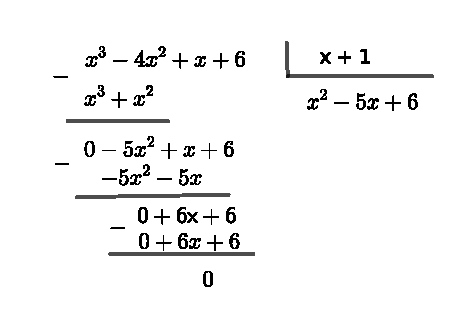
\includegraphics[width=8cm]{../Topicos/Figuras/polinomiosdivisao.pdf}
 \end{figure}
 
 note que o quociente da divisão é $q_1(x)= x^2 - 5x + 6$, e o resto desta divisão é $r(x)=0$ (zero). Como o resto é zero concluímos que $p_1(x)$ é divisível por $g_1(x)$. Portanto $p_1(x)= q_1(x)g_1(x)$, ou seja, $x^3-4x^2+x+6= (x^2-5x+6)(x+1)$.
 \end{exem}
 
 Como consequência do teorema anterior, temos o seguinte corolário, que nos garante que no exemplo anterior $-1$ é uma raiz do polinômio $p_1(x)$.
 
 \begin{cor}
 Seja $p$ um polinômio não-nulo sobre $K$. Seja $\alpha \in K$ tal que $p(\alpha)=0$. Então, existe um polinômio $q(x)$ sobre $K$ tal que 
 \[p(x)= (x - \alpha)q(x) \ .\]
 \end{cor}
 
 Como consequência deste Corolário, todo polinômio de grau $n \geq 1$ pode ser escrito como produto de $n$ fatores de grau $1$.
 
 \begin{teo}[Teorema da Decomposição]
  Todo polinômio $p(x)= a_nx^n + a_{n-1}x^{n-1}+ \ldots + a_1x+ a_0$, com $a_n \neq 0$, pode ser escrito de forma fatorada
  \[p(x)= a_n(x - r_1)(x - r_2) \ldots (x - r_n)\]
  onde $r_1, r_2, \cdots, r_n$ são as raízes do polinômio.  
 \end{teo}

